\documentclass[12pt]{article}
\usepackage[a4paper,margin=2.45cm]{geometry}
\usepackage[T1]{fontenc}
\usepackage[utf8]{inputenc}
\usepackage{lmodern}
\usepackage{microtype}
\usepackage{setspace}
\usepackage{amsmath,amssymb,bm,mathtools}
\usepackage{booktabs,tabularx,array,longtable}
\usepackage{graphicx}
\usepackage{tikz}
\usetikzlibrary{arrows.meta,positioning}
\usepackage{natbib}
\usepackage{xurl}
\usepackage{hyperref}
\usepackage{lineno}
\usepackage{enumitem}
\hypersetup{colorlinks=true,linkcolor=black,citecolor=black,urlcolor=blue}
\newcommand{\R}{\mathbb{R}}
\newcommand{\im}{\operatorname{im}}
\newcommand{\rankop}{\operatorname{rank}}
\newcommand{\card}[1]{\#\!\left\{#1\right\}}
\setlength{\emergencystretch}{3em}
\setlength{\parindent}{1.15em}
\setlength{\parskip}{0pt}
\doublespacing
\linenumbers
\pagestyle{plain}

\title{\textbf{Reproducible Hodge-Curl Relational Geometry of Conscious Visual Detection}}
\author{\parbox{0.94\textwidth}{\centering
Miroslav Sv\'itek$^{1,2,*}$\\[0.5em]
\small $^{1}$Czech Institute of Informatics, Robotics and Cybernetics at Czech Technical University in Prague, Czech Republic\\
\small $^{2}$Faculty of Natural Sciences, Matej Bel University, Slovakia\\
\small $^{*}$Corresponding author: Jugoslavskych partyzanu 1580/3, 160 00 Prague 6, Czech Republic\\
\small Email: [to be inserted before submission]}}
\date{Manuscript draft v0.6 -- 8 September 2026}

\begin{document}
\maketitle

\begin{abstract}
Conscious visual detection may depend not only on neural activity or coupling strength, but also on the geometry of time-directed relations across distributed neural signals. We formulate Spatiotemporal Geometric Information Theory (SGIT) by representing pairwise temporal relations as antisymmetric edge flows and decomposing them with Hodge theory into gradient, curl, and harmonic components. The primary observable is a temporal trajectory of normalized Hodge-curl modal energy, which measures how circulatory relational organization changes across time after total selected-mode magnitude has been removed. The trajectory was identified exploratorily in one visual-awareness dataset and then tested with the same frozen graph, basis, temporal windows, normalization, LOSO statistic, and inferential rule in an independent matched visual-threshold dataset. Primary inference used within-subject label permutations that recomputed all LOSO templates on every draw. The curl statistic exceeded its empirical permutation null in discovery ($p=0.0004$) and replication ($p=0.0064$), whereas the matched gradient representation remained unsupported. Effect sizes are small in absolute cosine-difference units (replication median $D\approx1.09\times10^{-5}$), but standardized descriptive effects are similar across datasets ($g_z=0.562$ and $0.575$). Because LOSO templates overlap across held-out subjects, $g_z$ is descriptive rather than an independent-subject inferential statistic. The results therefore provide reproducible evidence for a subtle group-level relational-geometric signature of conscious visual detection and define a quantitative target for future source-resolved and causal tests of SGIT.
\end{abstract}
\noindent\textbf{Keywords:} consciousness; visual awareness; EEG; Hodge Laplacian; Hodge-GFT; simplicial complex; relational dynamics; recurrent processing; geometric algebra

\section*{Significance Statement}
Consciousness research commonly measures neural activity, connectivity strength, or information quantity. SGIT tests a different property: the geometry of time-directed relations among neural signals. In two visual-threshold datasets, a circulation-sensitive Hodge trajectory showed the same direction of departure from a permutation null when the complete analysis was transferred without neural-outcome tuning, while a matched gradient representation remained unsupported. The raw LOSO cosine-difference scores are small and not uniformly positive across subjects, so the result should not be interpreted as a large individual-level biomarker. Its evidential basis is the full permutation procedure, which preserves the dependence created by overlapping LOSO templates. SGIT therefore contributes a reproducible group-level relational observable that can be localized and causally challenged in future experiments.

\section{Introduction}
The neuroscience of consciousness seeks neural properties that covary with conscious experience while remaining separable, as far as possible, from prerequisites, report processes, and consequences of awareness \citep{Aru2012,Koch2016,SethBayne2022}. Major theories emphasize different forms of organization. Global neuronal workspace theory stresses recurrent amplification and broad availability of information \citep{DehaeneChangeux2011}; recurrent-processing accounts emphasize recurrent and re-entrant interactions in sensory systems \citep{LammeRoelfsema2000,Lamme2006}; integrated information theory formalizes intrinsic causal structure and irreducibility \citep{Albantakis2023}. Recent adversarial comparisons reinforce a common requirement: theoretical claims must be converted into quantitative predictions that can be independently falsified \citep{Cogitate2025}.

Visual threshold paradigms are useful because physically similar stimuli can be followed by different subjective reports. A recurrent electrophysiological finding is visual awareness negativity (VAN), typically expressed around 200 ms over posterior electrodes, followed in many paradigms by later positive activity \citep{KoivistoRevonsuo2010,EklundWiens2018,Wiens2026}. Subjective scales such as the Perceptual Awareness Scale distinguish absence of experience from weak and clearer percepts \citep{RamsoyOvergaard2004,OvergaardSandberg2021}. These approaches have identified important neural correlates, but they usually quantify local amplitudes, latencies, connectivity strengths, or scalar information measures.

The present study asks a different question: \emph{how are time-directed relations among distributed neural signals geometrically organized?} Two neural states can have similar overall activity and similar total coupling while differing in whether their directed relations resemble potential-driven flow, local circulation, or larger topological cycles. Graph signal processing generalizes Fourier analysis to irregular networks \citep{Shuman2013}; topological and simplicial signal processing extend this idea to signals defined on edges and higher-order structures \citep{BarbarossaSardellitti2020,Schaub2021}. Hodge theory then provides an orthogonal decomposition of edge flows into gradient, curl, and harmonic components \citep{Jiang2011}.

We use this mathematics to formulate the empirical core of \emph{Spatiotemporal Geometric Information Theory} (SGIT). The tested principle is deliberately narrow: \textbf{conscious visual detection is associated with a reproducible temporal reorganization of the circulatory component of distributed neural relational geometry}. The claim is not that ``more curl'' means ``more consciousness''. The primary analysis removes total selected-mode energy and tests how normalized curl energy is redistributed across modes and time. Nor do we claim that Hodge curl is identical to biological feedback or that the measured signature is necessary, sufficient, or causal for consciousness.

The primary theoretical target is the transition from no reported visual experience to minimal conscious detection. This target was chosen because the source paradigms explicitly distinguish ``nothing'' from ``something'' or PAS1 from PAS2, and because prior ERP work suggests that detection awareness can differ from later identification awareness \citep{EklundWiens2018,Wiens2026}. SGIT therefore does not assume that the same circulation signature must increase monotonically with subjective clarity. A later \texttt{Something}$\rightarrow$\texttt{Identify} analysis was a separately frozen post-discovery generalization challenge, not an a priori component of the discovery hypothesis. Its role was to test whether the discovered detection signature generalized to a higher-level awareness transition; failure of that challenge narrows the empirical scope rather than retroactively redefining the original prediction.

The evidential design has three layers. Synthetic ground truth first tests whether the estimator separates curl topology, curl magnitude, and gradient structure. The human signature is then explored in one public visual-awareness dataset. Finally, the complete relational definition, graph, Hodge basis, selected modes, temporal windows, normalization, LOSO statistic, permutation algorithm, and decision threshold are transferred unchanged to an independent matched visual-threshold dataset. This frozen transfer, rather than the exploratory result alone, is the central replication test.

The contribution of SGIT in this paper is therefore specific. First, it defines a deterministic relation-first observable: a normalized Hodge spectral trajectory of chronology-sensitive edge relations. Second, it tests that observable with a permutation procedure that recomputes the complete LOSO system and therefore respects the dependence introduced by shared templates. Third, it shows that the same curl-specific group-level departure from the null transfers to an independent matched dataset without neural-outcome tuning. The Discussion separates this reproducible empirical core from stronger claims about anatomy, causality, or a universal theory of consciousness.

\section{Methods and Materials}
\subsection{Mathematical formulation of SGIT}
\subsubsection{Notation and inferential roles}
Table~\ref{tab:notation} collects the symbols used repeatedly below. Indices have fixed roles: $i,j$ index nodes, $n$ time samples, $s$ subjects, $q$ experimental conditions, $k$ temporal windows, $m$ Hodge modes, and $b$ permutation draws. This separation is used throughout to avoid mixing mathematical coordinates with experimental design parameters.

\begin{table}[p]
\centering\small
\caption{Core SGIT notation. Symbols introduced only locally are defined in the sentence or equation where they first appear.}
\label{tab:notation}
\begin{tabularx}{\textwidth}{@{}lX@{}}
\toprule
Symbol & Meaning\\
\midrule
$N,E,T$ & numbers of graph nodes, oriented edges, and filled triangles\\
$x_i[n]$ & scalar signal at node $i$ and sample $n$\\
$\ell$ & discrete chronology lag; $\varepsilon$ is the numerical stabilizer in the edge relation\\
$f_{ij}[n]$, $\bm f[n]$ & antisymmetric relation on edge $(i,j)$ and the resulting edge vector\\
$B_1,B_2$ & node--edge and edge--triangle incidence matrices\\
$L_1,L_{\rm grad},L_{\rm curl}$ & Hodge 1-Laplacian and its gradient and curl components\\
$U_c,U_g$ & selected curl and gradient Hodge eigenvector matrices\\
$\lambda_m$, $\tau_\lambda$ & Hodge eigenvalue of mode $m$ and positive-eigenvalue tolerance\\
$M$ & number of selected modes per Hodge subspace; $K$ is the number of temporal windows\\
$W_k$, $\mathcal I_k$ & temporal window $k$ and its sample-index set\\
$\mathcal R_s^{(q)}$ & retained trials/observations for subject $s$ in condition $q$\\
$E_{s,m,k}^{(q)}$ & mean squared energy of selected mode $m$\\
$p_{s,m,k}^{(q)}$, $h_{s,m,k}^{(q)}$ & normalized modal-energy proportion and its square-root (Hellinger) coordinate\\
$\bm\Gamma_s^{(q)}$ & unit-normalized concatenated temporal Hellinger trajectory\\
$C(\bm a,\bm b)$ & cosine similarity between vectors $\bm a$ and $\bm b$\\
$D_s$ & subject-level symmetric LOSO matching score\\
$D_{\rm group}^{\rm obs}$ & observed median of $D_s$ across subjects; $D_{\rm group}^{(b)}$ is the corresponding median after permutation draw $b$\\
$N_{\rm perm}$, $p$, $\alpha$ & number of permutation draws, Monte Carlo permutation value, and decision threshold\\
$d_z,g_z$ & standardized subject-score summaries; descriptive only because LOSO templates overlap\\
$Z_{\rm null}$ & observed group median expressed in standard deviations of its empirical permutation null; descriptive only\\
$k_{\rm nn}$ & number of nearest neighbours used only for experimental graph construction\\
\bottomrule
\end{tabularx}
\end{table}
\subsubsection{Graph and edge-valued signal}
Let a fixed undirected graph be $G=(V,\mathcal E)$, where $V=\{1,\ldots,N\}$ is the set of nodes and $\mathcal E$ is the set of $E=|\mathcal E|$ edges. A scalar signal $x_i[n]$ is observed at node $i$ and discrete time index $n$. Standard graph Fourier analysis acts on the node vector $\bm x[n]\in\R^N$ \citep{Shuman2013}. SGIT instead constructs a chronology-sensitive relation between selected node pairs and therefore works primarily with an edge vector $\bm f[n]\in\R^E$. The graph topology is an external specification of the mathematical model; its concrete construction is not required for the definitions that follow.

Each undirected edge is assigned one algebraic orientation. The orientation is a bookkeeping convention, not a claim about biological direction. Once an orientation is chosen, the edge set can be written as ordered pairs $e=(i,j)$, and reversing an edge changes only the sign of the corresponding edge coordinate.

\subsubsection{Incidence matrices $B_1$ and $B_2$}
The node-edge incidence matrix $B_1\in\R^{N\times E}$ records which nodes are incident to each oriented edge. The symbol $(B_1)_{ve}$ denotes the entry in row $v$ (node $v$) and column $e$ (edge $e$). For an edge $e=(i,j)$ stored with orientation $i\rightarrow j$,
\begin{equation}
(B_1)_{ve}=\begin{cases}
-1,&v=i,\\
+1,&v=j,\\
0,&\text{otherwise}.
\end{cases}
\label{eq:B1}
\end{equation}
Thus $B_1\bm f$ is the discrete divergence of an edge field: it summarizes the net signed edge flow at every node.

To represent local circulation, the graph is extended to a simplicial complex by specifying a set $\mathcal T$ of $T=|\mathcal T|$ filled triangles (2-simplices). For an oriented triangle $[i,j,k]$ with $i<j<k$, its boundary is
\begin{equation}
\partial[i,j,k]=[j,k]-[i,k]+[i,j].
\label{eq:triangleboundary}
\end{equation}
The edge-triangle incidence matrix $B_2\in\R^{E\times T}$ stores these coefficients. Each column of $B_2$ therefore has three nonzero entries, with signs determined by whether the stored edge orientation agrees with the oriented boundary of the triangle. The fundamental consistency relation is
\begin{equation}
B_1B_2=0,
\label{eq:boundaryzero}
\end{equation}
which states that the boundary of a boundary is zero \citep{Jiang2011,Schaub2021}.

For example, if $e_{12}:1\to2$, $e_{13}:1\to3$, and $e_{23}:2\to3$, then
\[
B_1=\begin{bmatrix}
-1&-1&0\\
1&0&-1\\
0&1&1
\end{bmatrix},\qquad
B_2=\begin{bmatrix}1\\-1\\1\end{bmatrix}.
\]
The minus sign associated with $e_{13}$ occurs because the oriented triangle boundary $1\to2\to3\to1$ traverses that side as $3\to1$, opposite to the stored orientation $1\to3$.

\subsubsection{Hodge decomposition}
Two edge-space operators are defined from the incidence matrices,
\begin{equation}
L_{\mathrm{grad}}=B_1^{\top}B_1,
\qquad
L_{\mathrm{curl}}=B_2B_2^{\top},
\qquad
L_1=L_{\mathrm{grad}}+L_{\mathrm{curl}}.
\label{eq:hodgeops}
\end{equation}
$L_1\in\R^{E\times E}$ is the Hodge 1-Laplacian. The edge space decomposes orthogonally as
\begin{equation}
\R^E=\im(B_1^{\top})\oplus\im(B_2)\oplus\ker(L_1).
\label{eq:hodge_decomp}
\end{equation}
Here $\im(A)$ is the image (column space) of $A$, $\ker(A)$ is the null space of $A$, and $\oplus$ denotes an orthogonal direct sum. The three components have distinct meanings: $\im(B_1^{\top})$ contains gradient flows generated by node potentials; $\im(B_2)$ contains local circulations generated by filled triangles; and $\ker(L_1)$ contains harmonic flows that are simultaneously divergence-free and locally curl-free but may circulate around larger topological holes \citep{Jiang2011,BarbarossaSardellitti2020,Schaub2021}.

For a connected graph, $\rankop(B_1)=N-1$ because adding the same constant to every node potential does not change any edge difference. The rank of $B_2$ is determined by the number of linearly independent triangle boundaries; different triangles may generate dependent boundary vectors. The dimension of the harmonic subspace is therefore
\begin{equation}
\dim\ker(L_1)=E-\rankop(B_1)-\rankop(B_2).
\label{eq:harmdim_general}
\end{equation}

\subsubsection{Hodge-GFT modes and mode rank}
Because $L_{\mathrm{curl}}$ and $L_{\mathrm{grad}}$ are real symmetric positive-semidefinite matrices, each admits an orthonormal eigendecomposition. A curl mode satisfies
\begin{equation}
L_{\mathrm{curl}}\bm u_m^{(c)}=\lambda_m^{(c)}\bm u_m^{(c)},
\qquad \|\bm u_m^{(c)}\|_2=1,
\label{eq:eigencurl}
\end{equation}
and a gradient mode is defined analogously from $L_{\mathrm{grad}}$.

The vector $\bm u_m^{(c)}\in\R^E$ is an edge-space pattern: its $e$th component gives the loading of edge $e$ in curl mode $m$. The scalar $\lambda_m^{(c)}\ge0$ is the corresponding Hodge eigenvalue. It is not a temporal frequency in hertz. Rather, it indexes how the edge pattern varies relative to the topology encoded by $B_2$; larger positive eigenvalues represent higher Hodge frequencies within the curl subspace. The same interpretation applies to gradient eigenvectors and eigenvalues with $B_1$ \citep{BarbarossaSardellitti2020,Schaub2021}.

Only modes with positive eigenvalues above a numerical tolerance $\tau_\lambda>0$ are retained. Their eigenvalues are sorted from smallest to largest. In this paper, the term \emph{mode rank} means only the ordinal position in that sorted positive-eigenvalue list; it is unrelated to matrix rank. If a subspace contains $Q$ positive modes and $M$ modes are to be sampled approximately uniformly across the spectrum, the one-based ranks can be chosen by the deterministic rule
\[
r_m=1+\operatorname{round}\!\left(\frac{(m-1)(Q-1)}{M-1}\right),\qquad m=1,\ldots,M,
\]
with a deterministic floor-based fallback if rounding would create duplicate indices. This rule is an index-selection convention, not an inferential equation. The values of $Q$, $M$, $\tau_\lambda$, and the selected ranks are implementation parameters and are not part of the general Hodge-GFT definition.

Because an eigenvector has arbitrary sign, a deterministic sign convention can be imposed by locating the component with largest absolute value and multiplying the entire eigenvector by $-1$ if that component is negative. If an eigenvalue is degenerate, the basis inside its eigenspace is not unique; exact numerical replication then requires preserving the selected basis vectors themselves, not only the eigenvalues.

\subsubsection{Chronology-sensitive normalized edge relation}
For each node $i$, consider the two-sample vector
\[
\bm y_i[n]=\big(x_i[n-\ell],\;x_i[n]\big)^{\top},
\]
where $\ell\ge1$ is a discrete lag. For a node pair $i,j$, the determinant
\[
\det\!\begin{bmatrix}
x_i[n-\ell]&x_i[n]\\
x_j[n-\ell]&x_j[n]
\end{bmatrix}
=x_i[n-\ell]x_j[n]-x_j[n-\ell]x_i[n]
\]
is the signed area spanned by the two local vectors. Exchanging $i$ and $j$ reverses its sign, so the quantity is naturally antisymmetric. In exterior or geometric algebra, the same oriented area is represented by the coefficient of the wedge product $\bm y_i\wedge\bm y_j$ \citep{HestenesSobczyk1984,Lavor2018}. A related determinant/wedge formulation was previously used by \citet{Svitek2024GA} to represent pairwise and higher-order integration; SGIT applies the same antisymmetric geometric principle specifically to successive neural samples.

The normalized relation is
\begin{equation}
f_{ij}[n]=
\frac{x_i[n-\ell]x_j[n]-x_j[n-\ell]x_i[n]}
{\sqrt{\left(x_i^2[n-\ell]+x_i^2[n]\right)
\left(x_j^2[n-\ell]+x_j^2[n]\right)}+\varepsilon},
\label{eq:edgeflow}
\end{equation}
where $\varepsilon>0$ is a small numerical stabilizer. Apart from the stabilizer, Eq.~\ref{eq:edgeflow} is the signed sine of the angle between $\bm y_i[n]$ and $\bm y_j[n]$. It is antisymmetric, chronology-sensitive, bounded in magnitude by one, and invariant to independent positive rescaling of either local two-sample vector. Evaluating it on all oriented edges produces $\bm f[n]\in\R^E$.

The coefficients may also be written conceptually as a geometric-algebra bivector field,
\begin{equation}
\mathcal B[n]=\sum_{i<j} f_{ij}[n]~\bm e_i\wedge\bm e_j,
\label{eq:bivector}
\end{equation}
where $\bm e_i\wedge\bm e_j$ is an oriented basis bivector. Equation~\ref{eq:bivector} is a mathematical representation of the measured pair relation; the present analysis itself operates on $\bm f[n]$ and the Hodge operators.

\subsubsection{Projection, modal energy, and temporal trajectory}
Let $U_c\in\R^{E\times M}$ contain $M$ selected curl eigenvectors. The curl coefficients at time $n$ are
\begin{equation}
\bm c[n]=U_c^{\top}\bm f[n]\in\R^M.
\label{eq:projection}
\end{equation}
A matched gradient representation is obtained by replacing $U_c$ with a selected gradient basis $U_g$ of the same width $M$.

Suppose repeated observations are grouped by subject $s$, condition $q$, and temporal windows $W_k$, $k=1,\ldots,K$. Let $\mathcal R_s^{(q)}$ be the retained observations for subject $s$ in condition $q$, and $\mathcal I_k$ the sample indices in window $W_k$. The index $r$ runs over retained observations, and $c_{sr,m}[n]$ denotes the coefficient of selected mode $m$ for subject $s$, retained observation $r$, and sample $n$. The mean squared energy of mode $m$ is
\begin{equation}
E_{s,m,k}^{(q)}=
\frac{1}{|\mathcal R_s^{(q)}|\,|\mathcal I_k|}
\sum_{r\in\mathcal R_s^{(q)}}\sum_{n\in\mathcal I_k} c_{sr,m}^2[n].
\label{eq:modeenergy}
\end{equation}
Within each subject, condition, and window, the modal energies are normalized; $\mu$ below is a dummy summation index over the $M$ selected modes,
\begin{equation}
p_{s,m,k}^{(q)}=\frac{E_{s,m,k}^{(q)}}{\sum_{\mu=1}^{M}E_{s,\mu,k}^{(q)}},
\qquad
h_{s,m,k}^{(q)}=\sqrt{p_{s,m,k}^{(q)}}.
\label{eq:hellinger}
\end{equation}
The vector
\[
\bm h_{s,k}^{(q)}=\big(h_{s,1,k}^{(q)},\ldots,h_{s,M,k}^{(q)}\big)^{\top}\in\R^M
\]
is the square-root representation of the normalized mode-energy distribution. Since the $p$ values sum to one, $\|\bm h_{s,k}^{(q)}\|_2=1$. The square-root map is used because it embeds a probability vector on the simplex into the positive orthant of the unit sphere, where ordinary Euclidean geometry corresponds directly to Hellinger geometry; specifically, the squared Hellinger distance is one half of the squared Euclidean distance between the two square-root vectors \citep{Amari2016}. This choice is therefore geometric rather than a variance-stabilizing transformation. The preceding energy normalization removes total selected-mode energy in each window, so the statistic concerns the relative distribution of energy across modes rather than their common amplitude.

The temporal trajectory is formed by concatenating the $K$ window vectors,
\begin{equation}
\widetilde{\bm\Gamma}_s^{(q)}=
\begin{bmatrix}
\bm h_{s,1}^{(q)}\\
\vdots\\
\bm h_{s,K}^{(q)}
\end{bmatrix}\in\R^{KM},
\qquad
\bm\Gamma_s^{(q)}=
\frac{\widetilde{\bm\Gamma}_s^{(q)}}{\|\widetilde{\bm\Gamma}_s^{(q)}\|_2}.
\label{eq:trajectory}
\end{equation}
Thus each subject and condition is represented by one unit vector whose dimension is the number of selected modes multiplied by the number of temporal windows.

\subsubsection{LOSO cross-subject statistic}
To test cross-subject reproducibility without allowing a subject to contribute to its own reference pattern, SGIT uses a leave-one-subject-out (LOSO) construction. For held-out subject $s$, the notation $-s$ means \emph{all subjects except subject $s$}. For condition $q$, the unit-normalized LOSO template is
\begin{equation}
\bm\mu_{-s}^{(q)}=
\frac{\sum_{r\ne s}\bm\Gamma_r^{(q)}}
{\left\|\sum_{r\ne s}\bm\Gamma_r^{(q)}\right\|_2}.
\label{eq:losotemplate}
\end{equation}
LOSO is appropriate here because the claim concerns a reproducible condition geometry across subjects rather than a subject-specific fit \citep{Varoquaux2017,Ramirez2020}.

Let $N_s$ denote the number of evaluable subjects. Let $C(\bm a,\bm b)=\bm a^{\top}\bm b/(\|\bm a\|_2\|\bm b\|_2)$ denote cosine similarity. For two conditions $A$ and $B$, the subject and group statistics are
\begin{align}
D_s=\frac12\Big[&C(\bm\Gamma_s^{(B)},\bm\mu_{-s}^{(B)})-C(\bm\Gamma_s^{(B)},\bm\mu_{-s}^{(A)})\nonumber\\
&+C(\bm\Gamma_s^{(A)},\bm\mu_{-s}^{(A)})-C(\bm\Gamma_s^{(A)},\bm\mu_{-s}^{(B)})\Big],
\qquad
D_{\mathrm{group}}=\operatorname{median}_{s=1,\ldots,N_s}D_s.
\label{eq:lososcoregroup}
\end{align}
The first difference asks whether condition $B$ for subject $s$ is closer to the $B$ than the $A$ LOSO template; the second asks the symmetric question for condition $A$. Therefore $D_s>0$ means that both trajectories are, on average, closer to their matching condition templates; $D_s=0$ means no preference; and $D_s<0$ means a reversed mapping. The median is used as a robust group summary. Equation~\ref{eq:lososcoregroup} is a custom symmetric template statistic built on standard cross-validation principles, not a conventional classification-accuracy measure \citep{Varoquaux2017}.

\subsubsection{Permutation inference}
A parametric sampling distribution for $D_{\mathrm{group}}$ is not assumed. Under the null hypothesis that the two condition labels are exchangeable within each subject, the pair $(\bm\Gamma_s^{(A)},\bm\Gamma_s^{(B)})$ can be swapped independently for each subject. For permutation draw $b$, all LOSO templates and all subject scores are recomputed after these swaps, producing $D_{\mathrm{group}}^{(b)}$. This preserves the paired subject structure while destroying systematic condition assignment, following the exchangeability logic of permutation inference \citep{Winkler2014}.

With $N_{\rm perm}$ random permutation draws and a directional alternative in the positive direction, the Monte Carlo permutation value is
\begin{equation}
p=\frac{1+\#\{b:D_{\mathrm{group}}^{(b)}\ge D_{\mathrm{group}}^{\mathrm{obs}}\}}{N_{\rm perm}+1}.
\label{eq:permp}
\end{equation}
The symbol $\#$ means the number of permutation draws satisfying the inequality. Here $D_{\rm group}^{\rm obs}$ is the group median computed from the observed, unswapped labels, while $D_{\rm group}^{(b)}$ is the group median after permutation draw $b$. The $+1$ correction in numerator and denominator prevents a randomly sampled permutation test from reporting $p=0$ \citep{PhipsonSmyth2010}. The numerical values of $N_{\rm perm}$, the decision threshold $\alpha$, and all evaluability gates are experimental design choices specified in Section~2.2.

For descriptive scale interpretation, the distribution of subject scores can additionally be summarized by
\[
d_z=\frac{\overline D}{s_D},\qquad g_z=Jd_z,\qquad J=1-\frac{3}{4(N_s-1)-1},
\]
where $\overline D$ and $s_D$ are the mean and sample standard deviation of the $D_s$ values, and $J$ is the small-sample Hedges correction \citep{Lakens2013}. The $D_s$ values are not statistically independent: every held-out subject uses a template built from the other $N_s-1$ subjects, so different LOSO scores share most of their template data. Consequently $d_z$ and $g_z$ are descriptive scale summaries only and are not used for independent-subject inference. The primary inference is the permutation test in Eq.~\ref{eq:permp}; its null preserves this dependence because all LOSO templates are recomputed after every within-subject label swap.

A second descriptive quantity is
\[
Z_{\rm null}=\frac{D_{\rm group}^{\rm obs}-\overline D_{\rm null}}{s_{\rm null}},
\]
where $\overline D_{\rm null}$ and $s_{\rm null}$ are the mean and standard deviation of the empirical values $D_{\rm group}^{(b)}$. Thus $Z_{\rm null}$ expresses the observed group median in units of the empirical null standard deviation. It is a descriptive null-displacement measure; no Gaussian interpretation is assumed.

\subsubsection{Mathematical algorithm}
The complete SGIT mapping is
\[
\begin{aligned}
\text{node signals} &\rightarrow \text{oriented edge relation} \rightarrow (B_1,B_2) \rightarrow (L_{\mathrm{grad}},L_{\mathrm{curl}})\\
&\rightarrow \text{Hodge modes} \rightarrow \text{normalized modal spectra} \rightarrow \bm\Gamma\\
&\rightarrow D_s \rightarrow D_{\mathrm{group}} \rightarrow p.
\end{aligned}
\]
The mathematical construction is complete once the graph, lag, mode set, temporal windows, and inferential design are specified. Their numerical values are implementation choices rather than additional mathematical assumptions.

\begin{figure}[t]
\centering
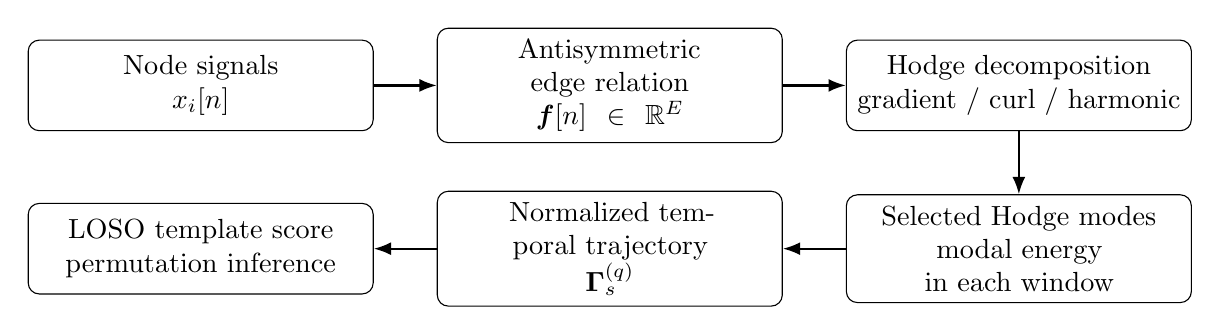
\begin{tikzpicture}[
box/.style={draw,rounded corners,align=center,text width=4.1cm,minimum height=1.15cm,inner sep=4pt},
arr/.style={-{Latex[length=2.2mm]},thick},
node distance=8mm and 8mm]
\node[box] (node) {Node signals\\$x_i[n]$};
\node[box,right=of node] (edge) {Antisymmetric edge relation\\$\bm f[n]\in\mathbb R^E$};
\node[box,right=of edge] (hodge) {Hodge decomposition\\gradient / curl / harmonic};
\node[box,below=of hodge] (modes) {Selected Hodge modes\\modal energy in each window};
\node[box,left=of modes] (traj) {Normalized temporal trajectory\\$\bm\Gamma_s^{(q)}$};
\node[box,left=of traj] (test) {LOSO template score\\permutation inference};
\draw[arr] (node) -- (edge);
\draw[arr] (edge) -- (hodge);
\draw[arr] (hodge) -- (modes);
\draw[arr] (modes) -- (traj);
\draw[arr] (traj) -- (test);
\end{tikzpicture}
\caption{SGIT analysis pipeline. Time-resolved node signals are converted to antisymmetric edge relations, decomposed in Hodge edge space, summarized as normalized modal-energy trajectories, and tested for cross-subject reproducibility with LOSO templates and within-subject label permutations. The diagram defines the logical sequence only; numerical experimental choices are specified in Section~2.2.}
\label{fig:pipeline}
\end{figure}

\subsection{Experimental implementation and data}
\subsubsection{Study logic, dataset independence, and ethics}
This work is a secondary analysis of publicly available de-identified EEG; no new participants were recruited and no new experimental data were collected. Participant recruitment, informed consent, and ethics procedures were conducted by the original investigators and are documented in the source publications \citep{EklundWiens2018,Wiens2026}. The present analysis used only public data and did not involve participant contact or re-identification.

The first human Hodge-GFT analysis was exploratory because the source dataset had already been accessed during theory development. After the exploratory curl result, the complete scientific analysis was frozen before the neural outcome of the replication dataset was evaluated. Here, \emph{independent} means a distinct source experiment with a non-overlapping participant dataset; it does not mean an independent laboratory, because both public datasets originated from the Stockholm University research environment. \emph{Matched} means that both analyses isolate the same conceptual detection boundary---no reported visual experience versus minimal reported visual experience---while allowing the stimuli, source preprocessing, file format, and sampling rate to differ. Technical file-reading amendments were permitted only when they changed neither the condition contrast nor any mathematical or inferential parameter.

Every experimental degree of freedom was either assigned a numerical value or generated by a deterministic rule. The discovery-derived channel order, nominal montage-coordinate table used for graph construction, oriented edge list, oriented triangle list, selected curl and gradient basis matrices, and selected mode ranks are supplied as Supplementary Data S1--S7. The independent replication used these exact discovery-derived graph and basis objects; it did not rebuild or rediagonalize a graph from the replication EEG.

\begin{table}[t]
\centering\small
\caption{Source datasets and their mapping to the SGIT detection contrast. ``Independent'' refers to distinct experiments and non-overlapping participant datasets, not to independent laboratories.}
\label{tab:datasets}
\begin{tabularx}{\textwidth}{@{}p{0.22\textwidth}XX@{}}
\toprule
 & Discovery & Frozen replication\\
\midrule
Source study & Wiens et al. (2026), Experiment 1 \citep{Wiens2026} & Eklund and Wiens (2018), LARGE-Gabor session \citep{EklundWiens2018}\\
Public data DOI & 10.17045/STHLMUNI.26879077 & 10.17045/STHLMUNI.5418967\\
SGIT evaluable $N$ & 30 & 35\\
Visual paradigm & thresholded detection/identification of digits and letters & thresholded low-contrast Gabors in four visual quadrants\\
Primary SGIT contrast & \texttt{Nothing} $\rightarrow$ UNSEEN; \texttt{Something} $\rightarrow$ SEEN & PAS1 (no experience) $\rightarrow$ UNSEEN; PAS2 (weak experience) $\rightarrow$ SEEN\\
EEG representation used by SGIT & 64 standard sensor labels; official preprocessed MNE/FIF epochs at 256 Hz & exact same 64 frozen sensor labels selected from source final FieldTrip data at 250 Hz\\
Source preprocessing & original K17/MNE preprocessing; no additional SGIT filtering or rereferencing & original authors' final FieldTrip preprocessing; no additional SGIT filtering, rereferencing, interpolation, or resampling\\
Independence from discovery & exploratory source dataset & distinct experiment and participants; same institution/research environment, different stimuli and source processing\\
\bottomrule
\end{tabularx}
\end{table}

\subsubsection{Exploratory discovery dataset}
The discovery data are Experiment 1 of \citet{Wiens2026}, with open data archived by Stockholm University \citep{WiensData2026}. The original study investigated electrophysiological correlates of detection and identification awareness for digits and letters and reported VAN in the established posterior awareness time range. The public Experiment-1 dataset contained 30 candidate participants, divided between digit and letter stimulus groups. The source experiment used 64 standard scalp channels; SGIT analyzed the official preprocessed K17 MNE epoch files at 256 Hz and did not reopen or reprocess the raw acquisition. No raw EEG fallback was used.

Only trials with source condition \texttt{detect} entered the primary SGIT detection contrast. Source response \texttt{Nothing} was mapped to UNSEEN and \texttt{Something} to SEEN. Source responses \texttt{Identify} and \texttt{Clear} were not merged with SEEN. Consecutive detection trials were partitioned into source-order chunks of 16 before official bad-EEG exclusion; a chunk was threshold-valid when 6--10 of its 16 responses were awareness-positive according to the source rule ``response $\ne$ Nothing''. Official bad trials were then excluded. At least 25 primary trials were required for each of UNSEEN and SEEN for a subject to be evaluable, and at least 24 evaluable subjects were required for the group test. These were design-specific evaluability gates.

\subsubsection{Independent matched replication dataset}
The replication used the preregistered visual-awareness dataset of \citet{EklundWiens2018}, with public data archived by Stockholm University \citep{EklundWiensData2018}. The original experiment presented low-contrast Gabor patches in four visual quadrants, with stimulus contrast calibrated to each participant's awareness threshold. Large and small Gabors were tested in separate sessions. The replication target was fixed to the LARGE-Gabor session only.

Only critical trial condition codes 1--4 were eligible. Subjective response 1 (PAS1: no visual experience) was defined as UNSEEN; subjective response 2 (PAS2: weak visual experience) was defined as SEEN; PAS3 was excluded from the primary contrast and was never pooled with PAS2. A behavioral feasibility audit identified 35 candidate LARGE-session participants with at least 25 PAS1 and 25 PAS2 critical trials before neural outcome analysis. This differs from the original paper's final LARGE-Gabor ERP sample of 24 because the present secondary analysis used its own prospectively frozen SGIT inclusion and quality-control rules.

The primary neural source was the original authors' final preprocessed individual FieldTrip data. The exact 64 discovery channel names had to be present. The files contained one additional channel, \texttt{Nz}; a technical amendment fixed before any Hodge outcome selected the exact 64 frozen names in frozen order and ignored only the extra \texttt{Nz} channel. The replication used source-native 250 Hz sampling; resampling to the discovery rate was not performed.

\subsubsection{Frozen sensor-space complex}
The graph was not inferred from EEG amplitudes. No subject-specific electrode location was estimated from the neural signals and no cortical source location entered graph construction. For graph construction only, each of the 64 discovery channel labels was associated with a fixed three-coordinate montage value available in the preprocessing metadata. The discovery implementation recorded this coordinate source as \texttt{FIF\_LOC}. These values are treated here solely as nominal sensor-layout coordinates used to define neighbourhood relations; they are not interpreted as participant-specific measured electrode positions or anatomical brain locations.

Let these fixed construction coordinates be $\widetilde{\bm p}_i\in\R^3$. Their Euclidean separation is
\begin{equation}
d_{ij}=\|\widetilde{\bm p}_i-\widetilde{\bm p}_j\|_2.
\label{eq:exp_distance}
\end{equation}
For every channel $i$, the six channels with smallest $d_{ij}$ were selected; $\mathcal N_6(i)$ denotes this directed set of six nearest neighbours of node $i$. This produces $64\times6=384$ \emph{directed neighbour selections}. The scale parameter $\sigma$ was defined as the median of these 384 selected distances,
\[
\sigma=\operatorname{median}\{d_{ij}:j\in\mathcal N_6(i),\ i=1,\ldots,64\}.
\]
Thus a reciprocal neighbour pair contributes twice to this median, once from each directed selection. In the frozen construction $\sigma=0.0378799070$ in the coordinate units of the supplied montage table. Positive provisional weights were then assigned by $w_{ij}=\exp[-d_{ij}^2/(2\sigma^2)]$ and symmetrized by union; only whether $w_{ij}>0$ determined the unweighted Hodge topology.

Among the 384 directed selections, 162 neighbour pairs were reciprocal (accounting for 324 directed selections) and 60 were one-sided. Their undirected union therefore contained $162+60=222$ unique edges. Each edge was assigned the deterministic algebraic orientation from smaller to larger node index. Every three-clique of this graph was filled as a triangle, producing 216 oriented 2-simplices. Hence the experimental Hodge complex contained
\[
N=64,\qquad E=222,\qquad T=216.
\]

The graph is connected, so the general identity $\rankop(B_1)=N-1$ gives $\rankop(B_1)=63$. For the actual $222\times216$ edge-triangle incidence matrix, direct rank evaluation gives $\rankop(B_2)=153$. The 216 triangle boundaries are therefore not linearly independent: $216-153=63$ independent combinations lie in $\ker(B_2)$ and do not add new curl directions. Consequently the edge space contains 63 independent gradient directions, 153 independent curl directions, and
\begin{equation}
\dim\ker(L_1)=222-63-153=6
\label{eq:exp_harmdim}
\end{equation}
harmonic directions. The exact edge and triangle lists and exact incidence-derived objects are supplied in Supplementary Data S2, S3, and S7.

\subsubsection{Frozen Hodge-GFT parameterization}
The positive-eigenvalue tolerance was $\tau_\lambda=10^{-9}$. The experimental complex contained 153 positive curl modes and 63 positive gradient modes. The analysis used $M=12$ modes from each subspace. Twelve was fixed during exploratory theory construction to provide a compact spectrum spanning low, middle, and high Hodge frequencies while preserving the same dimensionality for curl and gradient controls; it was not optimized against the replication outcome.

Applying the deterministic rank-selection rule from Section~2.1 gave the one-based curl ranks
\[
\{1,15,29,42,56,70,84,98,112,125,139,153\}
\]
and the one-based gradient ranks
\[
\{1,7,12,18,24,29,35,40,46,52,57,63\}.
\]
One selected curl eigenvalue belongs to a degenerate eigenspace, so the exact numerical $222\times12$ curl and gradient basis matrices were frozen after discovery and transferred unchanged to replication. They are supplied as Supplementary Data S4 and S5; the rank table is S6.

The chronology-sensitive edge relation used lag $\ell=1$ sample and stabilizer $\varepsilon=10^{-12}$, with numerical clipping to $[-1,1]$ only to suppress floating-point excursions. At 256 Hz the lag corresponds to 3.90625 ms; at the source-native 250 Hz replication rate it corresponds to 4 ms. The discrete one-sample lag, not the physical duration, was the frozen parameter.

The temporal representation used $K=3$ non-overlapping post-stimulus windows,
\[
W_1=[0.08,0.24),\qquad W_2=[0.24,0.40),\qquad W_3=[0.40,0.56)~\mathrm{s}.
\]
With $M=12$ modes and $K=3$ windows, each condition trajectory $\bm\Gamma_s^{(q)}$ had dimension $KM=36$.

\begin{table}[t]
\centering\small
\caption{Experimental SGIT parameters fixed for the human Hodge-GFT analysis. Mathematical symbols are defined in Section~2.1.}
\begin{tabularx}{\textwidth}{@{}l l X@{}}
\toprule
Quantity & Value & Experimental meaning\\
\midrule
$N,E,T$ & $64,222,216$ & nodes, oriented edges, filled triangles\\
${k_{\rm nn}}$ & 6 & nearest neighbours per channel before union symmetrization\\
$\sigma$ & 0.0378799070 & median of the 384 directed selected-neighbour distances\\
$\rankop(B_1),\rankop(B_2)$ & $63,153$ & independent gradient and triangle-boundary directions\\
$\dim\ker L_1$ & 6 & harmonic edge-space dimension\\
$\tau_\lambda$ & $10^{-9}$ & positive-eigenvalue tolerance\\
$M$ & 12 per subspace & selected curl modes and matched gradient modes\\
$\ell$ & 1 sample & discrete chronology lag\\
$\varepsilon$ & $10^{-12}$ & edge-relation numerical stabilizer\\
$K$ & 3 & number of temporal windows\\
$W_1,W_2,W_3$ & 80--240, 240--400, 400--560 ms & post-stimulus windows\\
$N_{\rm perm}$ & 9999 & within-subject condition-swap permutations\\
$\alpha$ & 0.025, one-sided & frozen support threshold\\
minimum trials & 25 per primary condition & subject evaluability gate\\
minimum subjects & 24 & group evaluability gate\\
\bottomrule
\end{tabularx}
\label{tab:experimental_parameters}
\end{table}

\subsubsection{Rationale for fixed graph, modes, lag, and windows}
The fixed parameterization was designed to minimize outcome-dependent model selection rather than to claim that one topology is uniquely optimal. The six-neighbour graph was chosen before the human Hodge outcome as a sparse local sensor graph: it preserves locality, remains connected in the frozen 64-channel montage, and generates enough 3-cliques to define a non-trivial curl subspace without using a dense all-to-all complex. Nearest-neighbour graph construction is a standard way to encode local geometry, although spectral results can in general depend on graph construction choices \citep{vonLuxburg2007}. No awareness label or EEG outcome entered the choice of $k_{\rm nn}=6$.

The 12 curl modes were not selected by energy, condition contrast, or predictive performance. They were sampled at approximately evenly spaced positive-eigenvalue ranks from the complete curl spectrum; the 12 gradient modes were chosen by the same rule. Thus the subsequent ``sum-to-one'' normalization is not circular with respect to mode selection. The one-sample lag was the minimal non-zero discrete lag capable of encoding temporal orientation in Eq.~\ref{eq:edgeflow}. Because the source-native rates were 256 and 250 Hz, the same frozen discrete rule corresponded to 3.906 and 4.000 ms, respectively, providing a small physical-time perturbation without retuning. The three 160-ms windows were fixed during theory construction before the Hodge human outcome and span early/VAN-range, intermediate, and later post-stimulus processing.

No post-hoc Delaunay, distance-threshold, alternative-$k_{\rm nn}$, alternative-mode-count, lag-2/3, or shifted-window sweep was performed on the successful datasets. Such a sweep after observing the primary result would add outcome-conditioned researcher degrees of freedom and would no longer be an independent confirmation. The robustness established here is therefore \emph{transfer robustness of one fully specified operator} across distinct datasets, stimuli, preprocessing pipelines, and nearby sampling rates, not invariance to every admissible graph or temporal parameter. A preregistered third-dataset sensitivity study is the appropriate test of parameter-family robustness.

\subsubsection{Dataset-specific preprocessing and nuisance control}
The relational algorithm after source preprocessing was identical across datasets. For discovery, the official preprocessed K17 epochs were used without additional filtering or rereferencing. For replication, the official Eklund--Wiens final files reflected the source pipeline described by the original authors: continuous 0.1-Hz fourth-order two-pass Butterworth high-pass filtering, downsampling to 250 Hz, epochs from -0.1 to 0.6 s around photodiode-validated onset, bad-channel handling/interpolation, ICA-based blink-component removal, average reference, baseline correction, and retention of rejected trials as non-finite values where appropriate \citep{EklundWiens2018}. SGIT added no filter, rereference, interpolation, or resampling to these final files.

Within each subject, baseline standardization used $[-0.09,0)$ s. For each sensor, the mean and standard deviation were estimated across all label-blind fit trials and all baseline samples; the complete epoch was then transformed by subtracting that mean and dividing by that standard deviation. A sensor baseline standard deviation below $10^{-8}$ was a technical failure.

Nuisance residualization was label-blind. At every sensor and time sample, trial amplitudes were regressed on a design matrix and residuals were retained. If $\bm y$ is the trial vector at one sensor-time point and $X$ the nuisance design, the residual is $\bm y-X(X^{+}\bm y)$, where $X^{+}$ is the Moore--Penrose pseudoinverse. In discovery, $X$ contained an intercept, valid-chunk-centered physical stimulus level, stimulus-identity dummy variables when at least two levels were present, and objective correctness when uniquely resolvable from source fields. The fit used all retained valid detection trials, including non-primary awareness responses. In replication, $X$ contained an intercept, critical condition code 1--4 as categorical dummy variables, and objective correctness; all finite critical PAS1/PAS2/PAS3 trials entered the nuisance fit. The subjective UNSEEN/SEEN label was never a nuisance regressor.

For replication, a trial passed technical finite-data QC only if every required sample from -0.09 through 0.56 s was finite in all 64 frozen channels. PAS1 and PAS2 then each had to retain at least 25 trials. Selection based on the original published final participant subset, Hodge outcome, or post-hoc edge, mode, lag, or window alternatives was not permitted.

\subsubsection{Synthetic validation and inferential protocol}
Before the human Hodge analysis, the estimator had to satisfy synthetic ground-truth gates that separated topology from simple magnitude. A synthetic curl-topology difference had to produce median LOSO score at least 0.25. A curl magnitude-only manipulation had to remain within absolute median 0.10. A gradient-only manipulation had to remain within absolute curl median 0.10 while producing gradient median at least 0.20. These tests verified that the numerical pipeline responded to the intended Hodge component; they were not biological EEG models. The frozen synthetic seed was 90520271.

For discovery, the sole primary human test was the median curl LOSO score with $N_{\rm perm}=9999$ within-subject condition swaps, seed 90520270, and a frozen directional threshold $\alpha=0.025$. The alternative was directional because the score itself was defined so that correct condition-template matching gives $D_{\rm group}>0$; a negative value represents systematic reversal rather than the same hypothesized signature with opposite sign. The value 0.025 was a conservative pre-outcome threshold, not a post-hoc Bonferroni correction. Curl was the primary subspace; the matched gradient analysis was a secondary specificity control and was not a co-primary test. Discovery and replication were sequential studies rather than simultaneous members of one multiplicity family. To make the directional assumption transparent, two-sided permutation values based on $|D_{\rm group}|$ are also reported as a sensitivity analysis in Results.

Support required technical PASS, at least 24 evaluable subjects, $D_{\rm group}>0$, and permutation $p\le0.025$. With 9999 random permutations and the $+1$ correction in Eq.~\ref{eq:permp}, the smallest attainable Monte Carlo value is $1/10000=0.0001$, and $p\le0.025$ corresponds to at most 249 permuted group statistics at least as large as the observed statistic. The stochastic uncertainty of a random-permutation estimate was quantified from the observed exceedance count with an exact binomial 95\% interval; this evaluates how much a different random seed could change the Monte Carlo tail estimate under the same null \citep{PhipsonSmyth2010}. An exact sign test on the number of $D_s>0$ subjects was reported independently as a secondary robustness statistic.

Because the datasets were fixed third-party resources, their sample sizes were not selected by an a priori power calculation for SGIT. Moreover, the primary LOSO median-permutation statistic has no simple closed-form power function. For orientation only, a conventional one-sample Gaussian score test at one-sided $\alpha=0.025$ would require approximately $|d|=0.53$ at $N=30$ and $|d|=0.49$ at $N=35$ for 80\% power; these are not power values for the primary permutation test. We therefore emphasize the full subject-score distributions, standardized descriptive effect sizes, permutation-null displacement, and independent replication rather than post-hoc observed-power estimates \citep{Lakens2013}.

After discovery, the independent replication transferred unchanged the 64-channel order, 222-edge graph, 216 triangles, exact 12-vector curl and gradient bases, one-sample lag, three windows, Hellinger normalization, LOSO statistic, permutation algorithm, direction of inference, and $\alpha=0.025$. The replication permutation seed was 90520274. The same support rule was fixed before neural outcome evaluation. Within-dataset trial split-half reliability was not part of the frozen result archive and is not introduced retrospectively here because defining a new halving rule after observing the outcome would itself constitute an additional analysis choice; reliability is instead evaluated by the independent dataset replication and by Monte Carlo precision of the permutation tail.

\section{Results}
\subsection{Synthetic validation recovered the intended topology}
All pre-specified synthetic sanity gates passed. When the synthetic ground truth changed curl topology, the median curl LOSO score was 0.6013, above the required 0.25. A magnitude-only curl manipulation produced a median essentially equal to zero, approximately $-2.7\times10^{-7}$, satisfying the absolute 0.10 null gate. A gradient-only manipulation likewise produced essentially zero curl score, approximately $-1.9\times10^{-7}$, while the matched gradient score was 0.6020, above the required 0.20. Thus the estimator could distinguish a change in circulatory topology from a change in overall magnitude and could separate curl from gradient structure before the human inference was interpreted.

\begin{table}[t]
\centering
\caption{Synthetic ground-truth validation. Gates were fixed before human Hodge outcome analysis.}
\label{tab:synthetic}
\small
\begin{tabularx}{\textwidth}{@{}lXrr@{}}
\toprule
Synthetic manipulation & Intended interpretation & Observed median & Gate\\
\midrule
Curl-topology change & pipeline should detect changed circulatory organization & 0.6013 & $\ge0.25$\\
Curl magnitude only & normalization should suppress pure magnitude change & $\approx0$ & $|D|\le0.10$\\
Gradient only, curl readout & curl should not respond to gradient-only structure & $\approx0$ & $|D|\le0.10$\\
Gradient only, gradient readout & matched gradient control should detect its own structure & 0.6020 & $\ge0.20$\\
\bottomrule
\end{tabularx}
\end{table}

\subsection{Exploratory discovery of a curl-trajectory signature}
All 30 discovery candidates were evaluable under the frozen gates. The primary curl analysis produced a median LOSO score of $7.626995\times10^{-5}$ and mean score $5.450092\times10^{-5}$; the standard deviation across subject scores was $9.4465\times10^{-5}$ and the interquartile range was $1.6273\times10^{-4}$. Nineteen of 30 individual scores were positive. Because $D_s$ is a difference between cosine similarities of unit-normalized 36-dimensional trajectories, its raw scale is necessarily small. Standardizing the subject-score mean by its own standard deviation gives descriptive $d_z=0.577$ and Hedges-corrected $g_z=0.562$ \citep{Lakens2013}. These standardized values are descriptive because LOSO scores share overlapping templates.

The permutation-null median was $8.6624\times10^{-7}$, its mean was $3.4291\times10^{-6}$, and its standard deviation was $1.5162\times10^{-5}$. The observed group median was therefore $Z_{\rm null}=4.80$ null standard deviations above the null mean. The null 97.5th percentile was $4.1878\times10^{-5}$. Only three of 9999 randomized within-subject label configurations produced a group median at least as large as the observed value, giving $p=(1+3)/10000=0.0004$. The exact binomial 95\% interval for the underlying exceedance probability corresponding to 3/9999 exceedances was approximately $6.2\times10^{-5}$ to $8.8\times10^{-4}$, far below the frozen $\alpha=0.025$; therefore ordinary Monte Carlo variation from changing the random seed would not plausibly change the support decision. A two-sided absolute-statistic permutation sensitivity analysis also gave $p=0.0004$.

The exact one-sided sign test was $p=0.1002$ (two-sided $p=0.2005$), so a simple majority-of-subjects test did not support the discovery effect. This is an important limit on individual-level interpretation: 19/30 subjects had $D_s>0$, but the effect was not uniform across subjects. The primary analysis asks a different group-level question and recomputes the complete dependent LOSO system under each within-subject label permutation. We therefore base inferential support on that permutation test and treat the positive-subject count, sign test, $d_z$, and $g_z$ as secondary diagnostics. The matched gradient analysis gave median $-6.8766\times10^{-6}$, mean $-8.0911\times10^{-6}$, descriptive $g_z=-0.219$, and 9/30 positive scores. Its directional permutation value was $p=0.7711$; the two-sided sensitivity value was $p=0.5271$. Thus the exploratory dataset did not show a generic change in both Hodge subspaces.

Because the discovery dataset had been accessed during theory development, this result was not treated as confirmatory evidence. Its scientific role was to define one exact candidate operator: the normalized curl trajectory, not total curl magnitude, should distinguish no reported visual experience from minimal reported visual experience in a new matched detection dataset.

\subsection{Independent frozen replication reproduced the curl signature}
All 35 behaviorally frozen replication candidates passed the neural QC rules. The smallest retained primary counts were 26 PAS1 trials and 71 PAS2 trials; no candidate was excluded for non-finite required samples or invalid shape. The analysis then used the exact discovery sensor-space graph and Hodge basis, with no reconstruction from the replication EEG.

The replication curl median was $1.087517\times10^{-5}$ and the mean was $1.274850\times10^{-5}$; the subject-score standard deviation was $2.1665\times10^{-5}$ and the interquartile range $3.2938\times10^{-5}$. Twenty-four of 35 subject scores were positive. The standardized descriptive effect was $d_z=0.588$ and Hedges-corrected $g_z=0.575$, closely matching the discovery standardized effect despite the smaller raw-score scale.

The replication null median was $1.9392\times10^{-7}$, null mean $6.5571\times10^{-7}$, and null standard deviation $3.1426\times10^{-6}$. The observed group median was therefore $Z_{\rm null}=3.25$ null standard deviations above the null mean. The null 97.5th percentile was $8.1844\times10^{-6}$. Sixty-three of the 9999 randomized label configurations reached or exceeded the observed statistic, yielding $p=(1+63)/10000=0.0064$. The exact binomial 95\% interval for the corresponding 63/9999 exceedance probability was approximately 0.00485--0.00805, again below $\alpha=0.025$. A two-sided absolute-statistic permutation sensitivity analysis also gave $p=0.0064$. As a secondary diagnostic, 24/35 subject scores were positive and the exact one-sided sign test gave $p=0.02048$ (two-sided $p=0.04096$). The frozen replication support rule was therefore satisfied by its primary permutation criterion; the sign test is reported separately and is not the basis for the standardized effect-size claim.

The matched gradient representation again remained unsupported. Its median score was $-1.1529\times10^{-6}$, mean $-1.1781\times10^{-6}$, descriptive $g_z=-0.145$, with 15/35 positive subject scores. The directional gradient permutation value was $p=0.7431$ and its two-sided sensitivity value was $p=0.5715$.

The independent result is the decisive evidence. The replication transferred the pre-specified graph, edge orientation, simplicial complex, numerical basis, lag, temporal windows, normalization, LOSO statistic, permutation algorithm, direction of inference, and alpha threshold. The source data differed in experiment, participants, stimuli, file format, preprocessing pipeline, and sampling rate. Because both source datasets came from the same institutional research environment, the replication is an independent dataset replication rather than an independent-laboratory replication.

\begin{table}[t]
\centering
\caption{Human Hodge-GFT results. The subject LOSO scores share overlapping templates and are therefore dependent. Accordingly, $g_z$ is a descriptive standardized summary only. Primary inference is the permutation $p$ value, which recomputes all templates after each within-subject label swap. $Z_{\rm null}$ is a descriptive displacement of the observed group median from its empirical permutation null.}
\label{tab:humanresults}
\small
\begin{tabularx}{\textwidth}{@{}lrrrrrr@{}}
\toprule
Analysis & $N$ & median $D$ & positive & $g_z$ & $Z_{\rm null}$ & perm. $p$\\
\midrule
Discovery curl & 30 & $7.6270\times10^{-5}$ & 19 & 0.562 & 4.80 & 0.0004\\
Discovery gradient & 30 & $-6.8766\times10^{-6}$ & 9 & -0.219 & -- & 0.7711\\
Replication curl & 35 & $1.0875\times10^{-5}$ & 24 & 0.575 & 3.25 & 0.0064\\
Replication gradient & 35 & $-1.1529\times10^{-6}$ & 15 & -0.145 & -- & 0.7431\\
\bottomrule
\end{tabularx}
\end{table}

\begin{figure}[t]
\centering
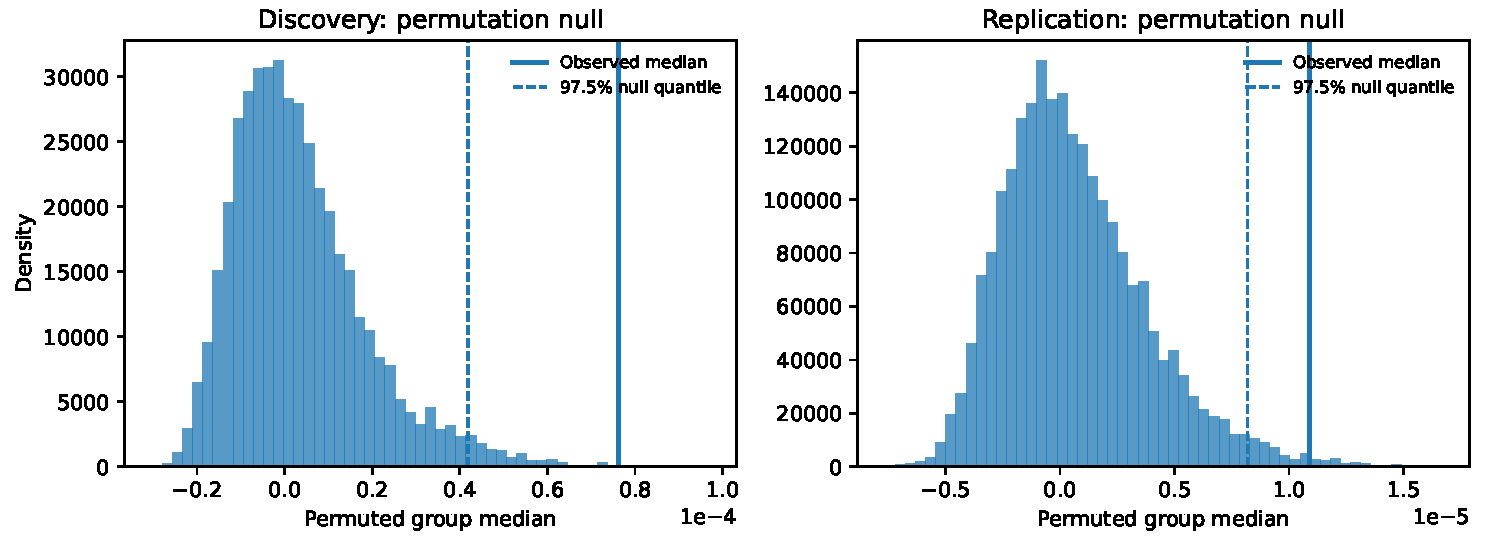
\includegraphics[width=0.98\textwidth]{figure2_permutation_nulls.pdf}
\caption{Permutation-null distributions for the primary curl group statistic. Left: discovery; right: frozen replication. The horizontal axis is $D_{\rm group}^{(b)}$, the median subject LOSO score obtained after permutation draw $b$; all LOSO templates are recomputed after each within-subject condition-label swap, so the null preserves the dependence created by overlapping templates. The bars show the empirical density of the 9999 permuted group medians. Solid vertical lines mark the observed unswapped medians $D_{\rm group}^{\rm obs}$ ($7.6270\times10^{-5}$ in discovery and $1.0875\times10^{-5}$ in replication); dashed lines mark the corresponding 97.5th null percentiles. Subject-level positive counts, sign tests, and descriptive $g_z$ values are reported in the text and Table~\ref{tab:humanresults}.}
\label{fig:effectdistributions}
\end{figure}

\subsection{Specificity, generalization boundary, and fixed-geometry null}
Two observations constrain the interpretation. First, the primary statistic is normalized within every time window before the temporal trajectory is formed. It cannot therefore be explained simply as greater total selected curl-mode energy in conscious trials. A secondary descriptive decomposition of total Hodge-subspace energy in the replication showed its largest SEEN-minus-UNSEEN curl-fraction shift in the late window, with median approximately $+0.00231$ and 25/35 positive subjects, while the gradient fraction shifted in the opposite direction (median approximately $-0.00212$). These quantities were not the primary inferential target.

Second, the \texttt{Something}$\rightarrow$\texttt{Identify} test was a separate post-discovery generalization challenge frozen before its own neural outcome; it was not an a priori prediction used to define the original detection discovery. The challenge asked whether the same operator generalized from the no-percept/minimal-percept boundary to a higher-level identification transition. It yielded 28 evaluable subjects, curl median $2.8264\times10^{-5}$ and $p=0.0296$, above the frozen $\alpha=0.025$; the gradient control also showed a weak trend at $p=0.0461$. The result is therefore negative under its frozen rule. It argues against describing the present curl trajectory as a universal ordinal marker that must accompany every increase in subjective awareness.

A further concern is that every subject is analyzed in the same sensor graph and Hodge basis. Shared geometry can create common cross-subject structure, but it is present identically under the observed labeling and under every within-subject label swap. The permutation null therefore preserves the common graph, basis, dimensionality, and the dependence induced by overlapping LOSO templates while destroying only the systematic assignment of condition labels. In discovery the null median was $8.66\times10^{-7}$ and in replication $1.94\times10^{-7}$, both close to zero relative to the observed curl medians. Thus the fixed graph does not by itself shift the condition-matching statistic away from zero under the tested exchangeability null. This does not prove invariance to alternative graph constructions; it quantifies the effect of the shared graph within the actual null hypothesis being tested.

\subsection{What is new in the replicated result}
The new observation is not simply that EEG differs between seen and unseen trials. SGIT changes the measured object: it tests the temporal geometry of a normalized, chronology-sensitive edge relation. The empirical contribution is that this exact construction shows a curl-specific group-level departure from its complete permutation null in discovery and again after frozen transfer to an independent matched dataset, while the matched gradient construction remains unsupported. Figure~\ref{fig:effectdistributions} shows the two primary permutation nulls directly.

The replication therefore supports a narrow statement: within the tested visual-threshold paradigms, conscious detection is reproducibly associated with a change in the temporal distribution of normalized Hodge-curl relational modes. The raw subject effects are small and heterogeneous, and the result is not an individual-level classifier. It does not show that curl generates consciousness, that the signature is universal, or that its scalp topology identifies the responsible cortical generators.

\section{Discussion}
\subsection{A reproducible relational-circulation signature of conscious detection}
The central finding changes the object being measured. Standard EEG contrasts ask whether activity, an ERP component, synchronization, or connectivity strength differs between conditions. SGIT first converts pairs of successive sensor samples into signed, normalized oriented areas and then asks how the resulting edge field occupies Hodge subspaces over time. The independent replication indicates that the geometry of these relations contains reproducible awareness information beyond a generic change in gradient organization.

This distinction is important because total magnitude is mathematically removed before the primary trajectory is compared. For every subject, condition, and time window, the 12 selected modal energies are normalized to sum to one. The subsequent square-root map and 36-dimensional concatenation therefore preserve the \emph{shape} of the modal distribution across time while suppressing a global scaling of selected-mode energy. The discovery and replication consequently support a statement about organization: the relative allocation of relational energy across curl modes evolves differently when a threshold stimulus is minimally experienced than when no visual experience is reported.

The absolute LOSO scores are small, especially in replication: the median was $1.0875\times10^{-5}$. They are also heterogeneous across subjects: 19/30 discovery and 24/35 replication scores were positive, and the discovery sign test was non-significant ($p=0.1002$, one-sided). These facts limit any claim of a large or uniform individual-level effect. In addition, the $D_s$ values are statistically dependent because each LOSO score uses a template formed from the other subjects and different held-out folds therefore share most template observations. For this reason $g_z$ is descriptive only, even though its values are similar across datasets ($0.562$ and $0.575$).

The inferential claim rests instead on the permutation test. Every label swap triggers a complete recomputation of all LOSO templates and subject scores, so the null distribution preserves the same overlap and dependence structure as the observed statistic. Under this null, the observed group median exceeded the 97.5th percentile in both discovery and frozen replication, with permutation $p=0.0004$ and $p=0.0064$, respectively. The supported effect is therefore best described as a subtle reproducible group-level geometry, not a large subject-level shift.

The repeated gradient result strengthens the geometrical interpretation. Gradient and curl belong to orthogonal Hodge subspaces with different topological meanings \citep{Jiang2011,BarbarossaSardellitti2020,Schaub2021}. In both human datasets, the curl trajectory met its inferential criterion while the matched gradient construction did not. This does not prove that gradient dynamics are irrelevant to consciousness. It shows only that the \emph{specific frozen representation that replicated} is circulation-sensitive rather than a generic property of any edge-space decomposition.

The negative identification-boundary generalization is equally informative. A useful theory should specify where its current evidence ends. The failed frozen \texttt{Something}$\rightarrow$\texttt{Identify} test argues against treating the present curl trajectory as a universal ordinal marker that simply increases with subjective clarity. One possible interpretation is that the identified geometry is more closely related to the transition from no percept to minimal conscious detection than to later identification, but that hypothesis requires new independent tests and is not established by the present data.

\subsection{Biological and anatomical interpretation}
The temporal organization is biologically plausible because the three fixed windows cover periods already implicated in visual awareness. The first window spans early visual processing and the canonical VAN range; VAN is commonly observed around 200 ms over posterior electrodes \citep{KoivistoRevonsuo2010,EklundWiens2018,Wiens2026}. The second and third windows extend through later recurrent, decision, and report-related processing in which positive ERP components are often observed. SGIT does not identify VAN or P3 as the measured object. Instead, it describes how distributed pair relations reorganize across a sequence that includes these established electrophysiological regimes.

Curl has an intuitive relation to recurrence, but the distinction between mathematical and biological language is essential. A Hodge-curl component is an edge-flow component lying in the image of $B_2$; it represents local circulation on the chosen simplicial complex. Biological recurrent processing refers to neuronal interactions that return information through cortical or thalamocortical pathways. Therefore Hodge curl is \emph{not} anatomical feedback, and Hodge gradient is \emph{not} feedforward anatomy. The repeated curl-specific result is nevertheless structurally compatible with theories in which conscious visual processing depends on recurrent or re-entrant organization rather than a purely feedforward sweep \citep{LammeRoelfsema2000,Lamme2006}.

The present statistic should also not be read as a subject-level diagnostic score: its validated inferential object is the group median under the recomputed permutation null.

The current data cannot localize that organization anatomically. Scalp EEG sensors measure mixtures of underlying cortical sources, and across-subject sensor correspondence does not imply identical cortical generators. This is particularly relevant for LOSO analyses, where shared measurement geometry can contribute to cross-subject structure \citep{Ramirez2020}. Our normalization removes simple selected-mode amplitude scaling and the exact sensor-space graph and basis are held fixed, but these steps do not solve the EEG inverse problem. Posterior or centro-parietal sensor loadings should therefore be described only as sensor-space topography, not as evidence that a particular cortical area generates the curl signature.

The biologically decisive extension is source-space testing. EEG or MEG could first be reconstructed to anatomically defined cortical parcels, after which Hodge relations could be defined among visual, parietal, frontal, or thalamocortical nodes. Intracranial recordings could test the same relational prediction with much less spatial mixing. These designs could ask whether awareness-related circulation first appears in posterior sensory circuits, whether it later couples to frontoparietal systems, or whether a different multiscale organization is required. Such tests would move SGIT from a reproducible sensor-space correlate toward an anatomically interpretable mechanism.

\subsection{Relation to theories of consciousness, robustness, and falsifiable interpretation}
SGIT is not proposed here as a replacement for established theories. None of recurrent-processing theory (RPT), global neuronal workspace theory (GNWT), or integrated information theory (IIT) explicitly predicts a Hodge-curl statistic. The useful comparison is therefore operational: each theory emphasizes a different form of neural organization, and SGIT supplies measurable geometric observables with which those emphases can be tested. Table~\ref{tab:theorypredictions} states these mappings as future discriminating predictions rather than retrospective claims of theoretical confirmation.

\begin{table}[t]
\centering\small
\caption{Theory-linked SGIT predictions. These are operational hypotheses for future tests; the established theories do not themselves define Hodge curl or gradient.}
\label{tab:theorypredictions}
\begin{tabularx}{\textwidth}{@{}p{0.18\textwidth}p{0.24\textwidth}Xp{0.18\textwidth}@{}}
\toprule
Framework & Organizational emphasis & SGIT operational prediction for a decisive future test & Current status\\
\midrule
RPT & recurrent/re-entrant sensory processing & source-resolved awareness should preferentially alter circulation-sensitive geometry in sensory/posterior recurrent circuits, especially near early awareness timing & qualitatively compatible; not anatomically tested\\
GNWT & recurrent amplification and global availability & later access/ignition should produce a broader large-scale geometric transition, potentially involving gradient, curl, and/or harmonic organization across frontoparietal networks & current detection result is not diagnostic\\
IIT & intrinsic causal structure and irreducibility & perturbational/source-level relational geometry should covary with independently computed causal-structure measures; sensor-space Hodge trajectories alone are insufficient & not tested by present data\\
\bottomrule
\end{tabularx}
\end{table}

RPT has the closest qualitative connection: a circulation-sensitive edge organization is a natural quantity to test when recurrent interactions are hypothesized to matter for conscious vision \citep{Lamme2006}. The present result supports compatibility, not identity. GNWT emphasizes recurrent amplification and broad availability of information \citep{DehaeneChangeux2011}; SGIT can ask whether such propagation is accompanied by gradient, curl, harmonic, or sequential combinations of these geometries. IIT emphasizes intrinsic cause-effect structure and irreducibility \citep{Albantakis2023}; the present Hodge trajectory is neither an integrated-information quantity nor an estimate of intrinsic causal power. Geometric algebra provides a language for oriented pairwise and higher-order relations \citep{HestenesSobczyk1984,Lavor2018,Svitek2024GA}, but the current bivector notation is representational rather than mechanistic.

The strongest robustness result in the present paper is exact transfer across datasets, not a retrospective hyperparameter sweep. The successful datasets differ in participants, visual material, source preprocessing, file representation, and sampling rate, while the mathematical operator was held fixed. This guards against outcome-driven retuning and shows that the effect is not confined to a single set of participants or one source-processing pipeline. It does not establish that $k_{\rm nn}=6$, $M=12$, lag one, or the three windows are uniquely correct. Alternative graph families, mode counts, lags, and windows should be evaluated prospectively on a third dataset, ideally with a factorial sensitivity design specified before outcome access. The absence of a post-hoc sweep is therefore both a limitation and a protection against overfitting.

Several other limitations define the present claim. The evidence is correlational and sensor-space; it cannot establish causality, necessity, sufficiency, or cortical source. Both successful human tests belong to visual threshold paradigms, so generalization to other modalities, spontaneous experience, sleep, anesthesia, or disorders of consciousness is unknown. The discovery was exploratory, making the independent frozen replication essential. Within-dataset split-half reliability was not part of the frozen archive, and the two source datasets came from the same institutional research environment. Finally, the unsuccessful identification generalization shows that the current signature should not be described as a universal consciousness metric.

These limitations make the theory testable rather than vague. The present licensed claim is: \emph{within visual threshold detection paradigms, conscious detection is reproducibly associated with a change in the temporal distribution of normalized Hodge-curl relational modes, whereas the matched Hodge-gradient organization does not show the corresponding effect}. Any future dataset that applies the frozen construction to the same type of contrast and repeatedly fails to reproduce the curl trajectory would weaken this empirical core. Conversely, source-space and perturbational replications would strengthen the biological interpretation.

\section{Conclusions and future directions}
This study identifies a reproducible group-level property of neural organization associated with conscious visual detection. The property is not the amplitude of an EEG component, the total strength of connectivity, or the total amount of curl energy. It is the temporal organization of a chronology-sensitive relational edge field after Hodge decomposition and within-window normalization. The raw LOSO cosine-difference scores are small, the subject effects overlap zero, and the discovery sign test is non-significant. Moreover, the LOSO scores are dependent because their templates overlap, so the similar standardized values ($g_z=0.562$ and $0.575$) are descriptive rather than inferential.

The evidential result is instead the complete group-level permutation test: all LOSO templates are recomputed under every within-subject label swap, and the observed curl median lies beyond the empirical null in both the exploratory dataset and the independently frozen replication. The matched gradient representation remains unsupported in both datasets. The replication therefore provides evidence for a subtle reproducible relational geometry while avoiding the stronger interpretation of a large or independent subject-level effect.

The result supports a relational circulation principle for the tested visual-detection transition: minimal conscious detection is associated with a reproducible reorganization of distributed curl-mode geometry. The evidence is specific enough to be falsifiable and limited enough to remain scientifically defensible. It does not show that curl is consciousness, that every conscious state has the same signature, or that the observed geometry causes experience. The failed cross-threshold identification generalization is an important boundary condition rather than an inconvenient exception.

The next stage of SGIT should therefore focus on biological localization and causal testing rather than on further retuning of the present datasets. Source-space EEG and MEG can place the same mathematics on cortical parcels and test posterior versus frontoparietal organization. Intracranial recordings can test whether comparable circulation appears in local and long-range neural populations with reduced volume-conduction ambiguity. Multiscale analyses can ask whether conscious detection depends on coordinated local and global cycles rather than a single sensor-scale complex. Cross-frequency variants can test whether the same relational geometry is expressed jointly across phase and amplitude dynamics.

A second direction is higher-order structure. The present study uses pairwise oriented relations, which can be represented as bivectors in geometric algebra. Future work can ask whether explicit triadic closure carries additional information and whether such triadic relations are usefully represented by trivectors, followed by higher-grade multivector descriptions. This extension is motivated by geometric algebra and previous determinant/wedge-product formulations of multi-component integration \citep{HestenesSobczyk1984,Lavor2018,Svitek2024GA}, but it remains a hypothesis until it produces pre-specified predictions that outperform the pairwise model on independent data.

A third direction is perturbation. If the replicated curl trajectory reflects a process relevant to conscious detection rather than a passive correlate, then interventions that selectively disrupt recurrent or relational organization should alter the trajectory and, under a stronger causal hypothesis, alter conscious experience. Transcranial stimulation, intracranial stimulation, pharmacological perturbation, or naturally occurring state changes could provide such tests when appropriate public or independently collected datasets are available.

The broader aim of SGIT is therefore not to replace established theories with another scalar measure. It is to provide a reproducible geometry in which competing neurobiological theories can make sharper predictions about how neural relations evolve. The present paper supplies an independently replicated empirical anchor for that programme: at the group level, conscious visual detection is associated with a temporally organized circulatory relational geometry that is not mirrored by the matched gradient representation. Whether this relational geometry generalizes across content, modality, scale, anatomy, and causal perturbation is now a concrete experimental question.

\section*{Acknowledgements}
This work was supported by the European Union under the project Robotics and advanced industrial production (No. CZ.02.01.01/00/22\_008/0004590) and by the Slovak Grant Agency VEGA (No. 1/0779/25).

\section*{Conflict of interest}
The author declares no conflict of interest.

\section*{Data availability}
The third-party datasets analyzed in this article are publicly available at \url{https://doi.org/10.17045/STHLMUNI.26879077} and \url{https://doi.org/10.17045/STHLMUNI.5418967}. The nominal montage-coordinate table used only for graph construction, the exact edge and triangle lists, selected curl and gradient basis matrices, mode-rank table, and complete frozen Hodge objects are included with this manuscript as Supplementary Data S1--S7. These supplementary numerical objects contain no participant EEG data. The original third-party EEG files are not redistributed. The exact frozen analysis scripts and configuration files used for the discovery and replication are retained with the revision archive; a public repository DOI has not yet been assigned and is therefore not claimed here.

\section*{Author contributions}
M.S.: Conceptualization, methodology, formal analysis, investigation, software, visualization, writing--original draft, and writing--review and editing.

\bibliographystyle{apalike}
\bibliography{references}
\end{document}
